%-------------------------------------------------------------------------------
\section{Introduction}
%-------------------------------------------------------------------------------
\label{sec:intro}
% With the widespread use of social networking services and other internet services, 
% Graph analytics is a useful tool to extract valuable statistics or 


Analysis of network statistics is a useful tool for finding meaningful patterns in graph data, such as social, e-mail,  citation and epidemiological networks. 
For example, the average \textit{degree} (i.e., number of edges connected to a node) in a social graph can reveal the average connectivity. 
% , and \textit{subgraph counts} 
\textit{Subgraph counts} 
(e.g., the number of triangles, stars, or cliques) can be used to measure 
centrality properties such as the \textit{clustering coefficient}, 
which represents the probability that two friends of an individual will also be friends of one another \cite{Newman_PRL09}. 
% of a graph. 
However, the vast majority of graph analytics is carried out on sensitive data, which could be leaked through the results of graph analysis. Thus, there is a need to develop solutions that can analyze these graph properties while still preserving the privacy of 
% individual people 
individuals 
in the network.

%While such graph statistics is important to understand the property of graphs, 
%graph analysis often raises a serious privacy concern. 
% the graphs often involve sensitive data; e.g., some users may not want to reveal her friend list to strangers. 
%For example, 
% a graph may involve 
%edges could correspond to sensitive friendships 
% or sexual relationships 
%that a user wants to keep secret. 
%User attributes (e.g.,  gender, profession, dormitory) might also be inferred from a social network \cite{Dougnon_AI15,Mislove_WSDM10}.
%Therefore, it is desirable to develop an algorithm for analyzing graph statistics while protecting user privacy.

% Privacy-preserving graph analysis 
The standard way to analyze graphs with privacy is through differentially private graph analysis \cite{Raskhodnikova_Encyclopedia16,DP,Dwork_ICALP06}. 
Differential privacy 
provides individual privacy against adversaries with arbitrary background knowledge, and has currently emerged as the gold standard for private analytics. 
However, a vast majority of differentially private graph analysis algorithms are in the \textit{centralized (or global) model} \cite{Blocki_FOCS12,Chen_PoPETs20,Day_SIGMOD16,Hay_ICDM09,Karwa_PVLDB11,Kasiviswanathan_TCC13,Nissim_STOC07,Raskhodnikova_arXiv15,Raskhodnikova_Encyclopedia16,Song_arXiv18,Wang_PAKDD13,Wang_TDP13}, where a single trusted data curator holds the entire graph and releases sanitized versions of the statistics. 
By assuming a trusted party that can access the entire graph, 
it is possible to release accurate graph statistics 
(e.g., subgraph counts \cite{Karwa_PVLDB11,Kasiviswanathan_TCC13,Song_arXiv18}, degree distribution \cite{Day_SIGMOD16,Hay_ICDM09,Raskhodnikova_arXiv15}, spectra \cite{Wang_PAKDD13}) 
and synthetic graphs \cite{Chen_PoPETs20,Wang_TDP13}. 

In many applications however, a single trusted curator may not be practicable due to security or logistical reasons. A centralized data holder is amenable to security issues such as data breaches and leaks -- a growing threat in recent years \cite{data_breach1,data_breach2}. Additionally, \textit{decentralized social networks} \cite{Paul_CN14,Salve_CSR18} (e.g., Diaspora \cite{Diaspora}) have no central server that contains an entire social graph, and use instead many servers all over the world, each containing the data of users who have chosen to register there.  Finally, a centralized solution is also not applicable to fully decentralized applications, where the server does not automatically hold information connecting users. An example of this is a mobile application that asks each user how many of 
% their 
her 
friends 
% they have 
she has 
seen today, and sends noisy counts to a central server. In this application, the server does not hold any individual edge, but can still aggregate the responses to determine the average mobility in an area. 

The standard privacy solution that does not assume a trusted third party is LDP (Local Differential Privacy) \cite{Duchi_FOCS13,Kasiviswanathan_FOCS08}. 
This is a special case of DP 
(Differential Privacy) 
in the \textit{local model}, where each user obfuscates her personal data by herself and sends the obfuscated data to a (possibly malicious) data collector. 
Since the data collector does not hold the original personal data, it does not suffer from data leakage issues. 
Therefore, LDP has recently attracted attention from both academia \cite{Acharya_AISTATS19,Bassily_STOC15,Bassily_NIPS17,Fanti_PoPETs16,Kairouz_ICML16,Kairouz_JMLR16,Murakami_USENIX19,Qin_CCS16,Wang_USENIX17,Ye_ISIT17} as well as industry \cite{Erlingsson_CCS14,Ding_NIPS17,Thakurta_USPatent17}. 
% Most of the studies on LDP focus on 
However, the use of LDP has mostly been in the context of tabular data where each row corresponds to an individual, and little attention has been paid to LDP for more complex data such as graphs (see 
Section~\ref{sec:related} for details). 
% Related work at the end of Section~\ref{sec:intro}). 

\begin{figure}
\centering
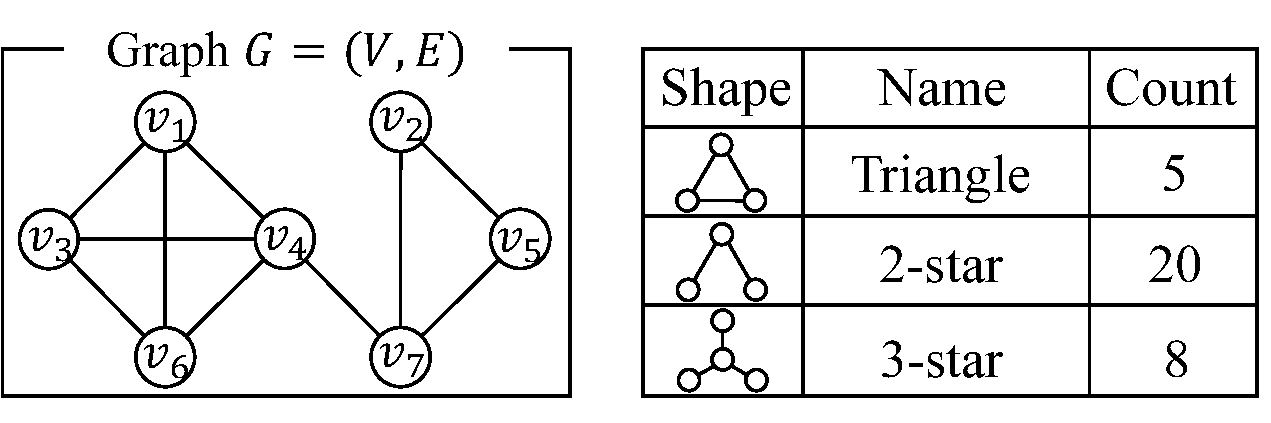
\includegraphics[width=0.9\linewidth]{fig/subgraph.pdf}
\vspace{-5.8mm}
\caption{Example of subgraph counts.}
\label{fig:subgraph}
\end{figure}

In this paper, we consider LDP for graph data, and 
% propose solutions 
provide algorithms and theoretical performance guarantees
for calculating graph statistics in this model. 
In particular, we focus on counting triangles and $k$-stars -- the most basic and useful subgraphs. 
% such as triangles and $k$-stars. 
A triangle is a set of three nodes with three edges (we exclude automorphisms; i.e., \#closed triplets $= 3 \times$ \#triangles). 
A $k$-star consists of a central node connected to $k$ other nodes. 
Figure~\ref{fig:subgraph} shows an example of triangles and $k$-stars. 
Counting them is a fundamental task of analyzing the connection patterns in a graph, as 
% measures of centrality such as 
the clustering coefficient can be calculated from triangle and $2$-star counts as: $\frac{3 \times \text{\#triangles}}{\#2\text{-stars}}$ (in Figure~\ref{fig:subgraph}, $\frac{3 \times 5}{20} = 0.75$). 

When we look to protect privacy of relationship information modeled by edges in a graph, 
we need to pay attention to the fact 
% Note 
that some relationship information 
% about friendship (edges) 
could be leaked from subgraph counts. 
For example, 
% consider an adversary who 
suppose that user (node) $v_2$ in Figure~\ref{fig:subgraph} knows 
all edges connected to $v_2$ and 
all edges between $v_3, \ldots, v_7$ 
as background knowledge, and that $v_2$ wants to know who are friends with $v_1$. 
Then ``\#2-stars = 20'' reveals 
% to $v_2$ 
the fact that $v_1$ has three friends, and ``\#triangles = 5'' reveals 
% to $v_2$ 
the fact that the three friends of $v_1$ are $v_3$, $v_4$, and $v_6$. 
Moreover, a central server that holds all friendship information (i.e., all edges) may face data breaches, as explained above. 
Therefore, a private algorithm for counting subgraphs in the local model is highly beneficial to individual privacy.

%Counting subgraphs in the local model is very challenging. 
The main challenge in counting subgraphs in the local model is that existing techniques and their analysis do not directly apply. 
The existing work on LDP for tabular data assumes that 
each person's data 
is independently and identically drawn from an underlying distribution. 
% (see Section~\ref{sec:related}). 
In graphs, this is no longer the case; e.g., 
each triangle is not independent, 
because multiple triangles can involve the same edge; 
each $k$-star is not independent for the same reason. 
Moreover, complex inter-dependencies involving multiple people 
% is 
are 
possible in graphs. 
For example, each user cannot count triangles involving herself, because she cannot see edges between other users; 
e.g., 
% in Figure~\ref{fig:subgraph}, 
user 
% (node) 
$v_1$ cannot see an edge between $v_3$ and $v_4$ in Figure~\ref{fig:subgraph}. 

% This simultaneously presents both challenges and opportunities. 
We show that although these complex dependency among users introduces challenges, it also presents opportunities. Specifically, this kind of interdependency also implies that extra interaction between users and a data collector may be helpful depending on the prior responses. 
In this work, we investigate this issue and provide algorithms for accurately calculating subgraph counts under LDP. 
% counts that use various levels of interaction. 

\smallskip
\noindent{\textbf{Our contributions.}}~~In this paper, we provide 
% To our knowledge, we are the first to provide 
algorithms and corresponding performance guarantees for counting triangles and $k$-stars in graphs under edge Local Differential Privacy. Specifically, our contributions are as follows:
\begin{itemize}
    \item For triangles, we present two algorithms. The first is based on 
    Warner's RR (Randomized Response) \cite{Warner_JASA65} 
    and empirical estimation \cite{Kairouz_ICML16,Murakami_USENIX19,Wang_USENIX17}. 
    We then present a more sophisticated algorithm that uses an additional round of interaction between users and data collector. We provide upper-bounds on the estimation error for each algorithm, and show that the latter can  significantly reduce the estimation error. 
    
    \item For $k$-stars, we present a simple algorithm using the Laplacian mechanism. We analyze the upper-bound on the estimation error for this algorithm, and 
    show that it is order optimal in terms of the number of users among all LDP mechanisms that do not use additional interaction.
    
    \item We provide lower-bounds on the estimation error for 
    %estimating 
    general graph functions including triangle counts and $k$-star counts in the local model. These are stronger than known upper bounds in the centralized model, and illustrate the limitations of the local model over the central.
    
    \item Finally, we evaluate our algorithms on two real datasets, and show that 
    it is indeed possible to accurately estimate 
    subgraph counts in the local model. 
    %Our experimental results show that 
    %although the algorithms in the local model provide high estimation errors than those in the centralized model,  
    In particular, we show that 
    the interactive algorithm for triangle counts and the Laplacian algorithm for the $k$-stars provide small estimation errors when the number of users is large.
\end{itemize}

We implemented our algorithms with C/C++, and published them as open-source software \cite{LDPGraphStatistics}.

% \smallskip
% \noindent{\textbf{Related work.}}~~Here we explain the previous work related ours. 
